\documentclass{article}
\usepackage[utf8]{inputenc}
\usepackage[T1]{fontenc}
\usepackage{polski}
\usepackage{indentfirst}
\usepackage{lastpage}
\usepackage{graphicx} 

\usepackage{fancyhdr}
\pagestyle{fancy}
\fancyhf{}
\rhead{Franciszek Wysocki, Bartosz Zdybel}
\rfoot{Strona \thepage \hspace{1pt} z \pageref{LastPage}}
\lhead{Spis treści}
\title{Sprawozdanie końcowe dla projektu pt. \\ ,,Gra w życie''}
\author{}
\date{}

\begin{document}
\maketitle

\begin{flushright}
\par ...
\vfill
\par
Wykonali: Franciszek Wysocki, Bartosz Zdybel

Sprawdzający: mgr inż. Paweł Zawadzki

Data: 30.03.2020
\end{flushright}

\thispagestyle{empty}
\newpage
\begin{frame}{}
    \tableofcontents
\end{frame}
\newpage
\lhead{Cel projektu}
\section{Cel projektu}
{\fontsize{14}{14}\selectfont
Celem projektu było napisanie programu symulującego automat komórkowy Johna Conwaya ,,Gra w życie'', który ponadto powinien umożliwić:
\begin{itemize}
\item wczytywanie danych z pliku,
\item przeprowadzenie zadanej przez użytkownika liczby operacji,
\item wygenerowanie N obrazów w formacie plików png,
\item zapisanie bieżącej lokalizacji do pliku,
\item działanie z dwoma rodzajami sąsiedztwa von Neumanna i Moore'a,
\end{itemize}

}
\lhead{Cel projektu}
\section{Struktura projetu}
{\fontsize{14}{14}\selectfont
Program, tak jak wcześniej założyliśmy, składa się z 7 modułów, (które są dokładnie opisane w specyfikacji implementacyjnej):
\begin{itemize}
\item main
\item control
\item input\_file
\item output\_file
\item board
\item png\_drawing
\item movement 
\end{itemize}
Program można skompilować przy użyciu Makefile, który pomaga również w kompilacji i uruchomieniu testów: test\_board.c, test\_control.c, test\_input\_file.c, test\_movement.c, test\_output\_file.c, test\_png\_drawing.c.

Dodaliśmy również element ,,help'', które pomoże użytkownikowi uruchomić poprawnie program.
}
\section{Różnice miedzy specyfikacjami}
{\fontsize{14}{14}\selectfont

Program w większości powstał z głównym planem opisanym szczegółowo w specyfikacjach.
\newline
\newline
Niemniej jednak niektóre zmiany zostały dokonane. Przede wszystkim w założeniach program nie miał prowadzić dialogu z użytkownikiem, a wszystkie parametry miały być podawane w wierszu poleceń np. w wersji oznaczonej tagiem \texttt{STABLE\_1.0}, flaga \texttt{-SBS} odpowiadała za wyświetlanie każdej iteracji po kolei, a żeby zwiększyć ilość iteracji należało ustawić odpowiedni parametr po fladze \texttt{-N}. Obecnie flaga \texttt{-SBS} jest niezależna, co daje jej dodatkową funkcjonalność dla poszczególnych iteracji (Rysunek 1).

\begin{figure}[h]
\centering
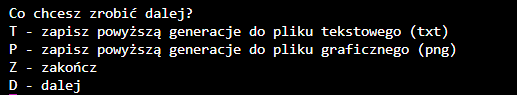
\includegraphics[width=10cm]{sbs.png}
\caption{}
\label{fig:obrazek }
\end{figure}


Druga zmianą jaką zastosowaliśmy w programie było dodanie funkcji ,,help'', która ma ułatwić użytkownikowi korzystanie z programu.


W programie postanowiliśmy również rozdzielić funkcjonalność flagi \texttt{-N}, która we wcześniejszych wersjach (np. \texttt{STABLE\_1.0}) przeprowadzała ,,n'' iteracji i generowała obraz png z każdego stanu, gdzie ,,n'' to parametr po tejże fladze. Uznaliśmy, że użytkownik może nie chcieć za każdym razem generować obrazów, dlatego, aby je wygenerować w finalnej wersji oprócz flagi -N, która po zmianie odpowiada jedynie za przeprowadzenie ,,n'' iteracji i wyświetlenie ich na standardowym wyjściu, należy dodać flagę \texttt{-PNG}.
Przykład: \texttt{ ./a.out -N 3 -PNG }



}

\lhead{Efekt działania}
\section{Efekt działania dla prawidłowych danych}
{\fontsize{14}{14}\selectfont

W celu prawidłowego uruchomienia programu należy przykładowo wpisać jedną z poniższych komend:


\textt{./a.out dane1.txt }

Jest to najbardziej podstawowa wersja uruchomienia. Program odczyta dane z podanego pliku, wykona jedną iterację i wyświetli na wyjściu standardowym generację inicjacyjną oraz powstałą (Rysunek 2).

\begin{figure}[h]
\centering
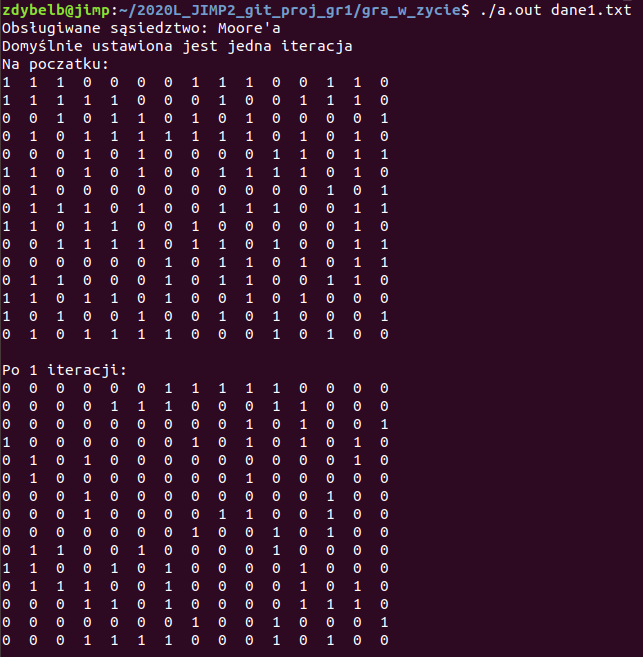
\includegraphics[width=10cm]{podstawowe.png}
\caption{}
\label{fig:podstawowe.png}
\end{figure}




\texttt{./a.out dane1.txt -N 5} 

W powyższych przypadku program odczyta dane z podanego pliku, wykona pięć iteracji i wypisze na wyściu standardowym generacje inicjacyjną oraz powstałe (Rysunek 3).


\begin{figure}[h]
\centering
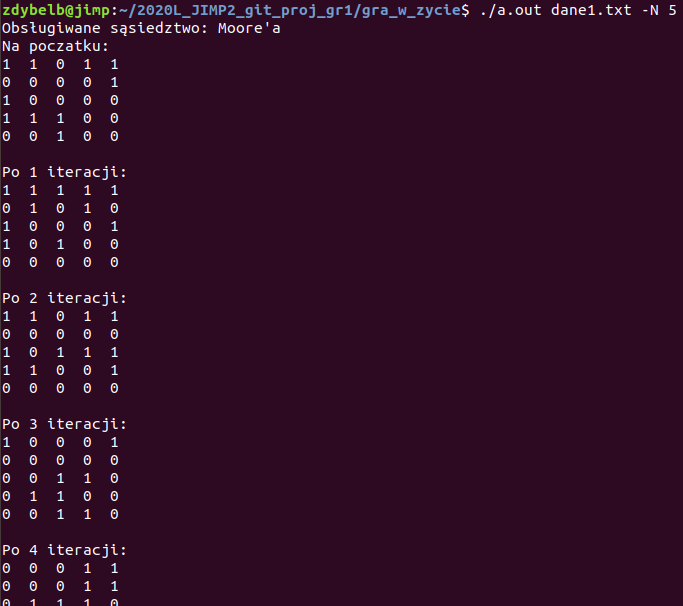
\includegraphics[width=10cm]{N.png}
\caption{}
\label{fig:N.png}
\end{figure}

\newpage

\textt{./a.out dane1.txt -N 3 -PNG}

Program odczyta dane z podanego pliku, wykona trzy iteracje i wypisze na wyjściu standardowym generacje inicjacyjną oraz powstałe, a następnie wygeneruje plik graficzny (png) dla każdej z nich (Rysunek 4).

\begin{figure}[h]
\centering
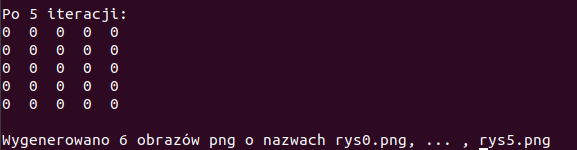
\includegraphics[width=10cm]{PNG.png}
\caption{}
\label{fig:PNG.png}
\end{figure}

\newline
\newline

\texttt{./a.out dane1.txt -S nowe\_dane.txt } 

Program odczyta dane z podanego pliku, wykona jedną iterację i wyświetli na wyjściu standardowym powstałą generacje oraz zapisze ją w pliku o podanej nazwie (w tym przypadku  nowe\_dane.txt). Można do tej komendy dodać flagi \texttt{-N} i \texttt{-PNG} (Rysunek 5).

\begin{figure}[h]
\centering
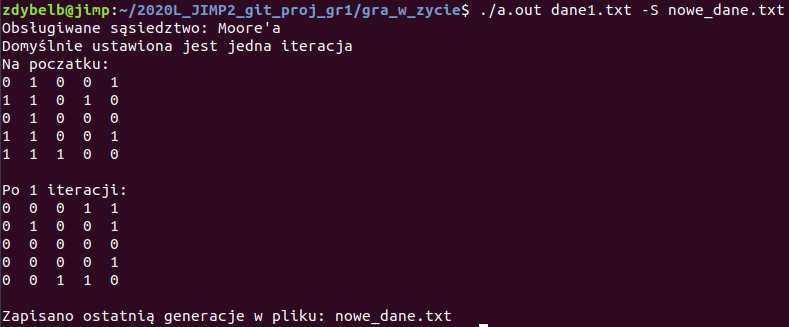
\includegraphics[width=10cm]{flagaS.png}
\caption{}
\label{fig:flagaS.png}
\end{figure}
\newline
\newline

\texttt{./a.out -H }

Uruchamia ,,helpa'', z którego można dowiedzieć się jak ma wyglądać plik wejściowy, pomoże użytkownikowi w poprawnym uruchomieniu programu oraz umożliwi sprawdzenie zwracanych wartości przez program, dzięki czemu będzie można sprawdzić jaki błąd spowodował zakończenie działania (Rysunek 6)
\newline
\begin{figure}[h]
\centering
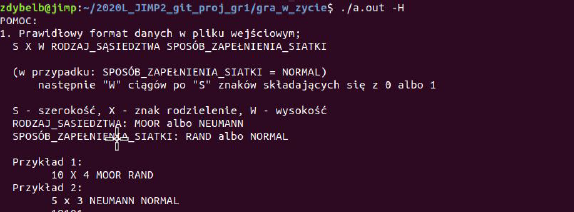
\includegraphics[width=12cm]{help.png}
\caption{}
\label{fig:help.png}
\end{figure}




\texttt{./a.out dane1.txt -SBS } 

W powyższym przypadku, program odczyta dane z podanego pliku i przejdzie w tryb dialogu z użytkownikiem (Rysunek 1). Dla każdej generacji ,,$N$'' można wygenerować plik tekstowy zapis$N$.txt, plik graficzny zapis$N$.png, pójść dalej (wyświetlić na wyjściu standardowym kolejną generację), bądź zakończyć.

\section{Poprawny format danych w pliku wejściowym}

\texttt{ S X W RS SZS }

\texttt{S} -  szerokość siatki,

\texttt{X} -  znak rozdzielenia (koniecznie znak X),

\texttt{W} -  wysokość siatki,

\texttt{RS} - obsługiwany ,,rodzaj sąsiedztwa'' (do wyboru \texttt{MOOR} lub \texttt{NEUMANN}),

\texttt{SZS} - obsługiwany ,,sposób zapełniania siatki'' (do wyboru \texttt{RAND} lub \texttt{NORMAL}),


RAND wymaga, aby nie było po nim żadnego argumentu, gdyż ciągi będą generowane losowo. NORMAL natomiast wymaga dokładnie \texttt{W} ciągów po \texttt{S} znaków (zer lub jedynek).

Przykład 1 (Rysunek 7):
\begin{figure}[h]
\centering
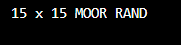
\includegraphics[width=4cm]{dobredane.png}
\caption{}
\label{fig:dobredane.png}
\end{figure}


Przykład 2 (Rysunek 8):
\begin{figure}[h]
\centering
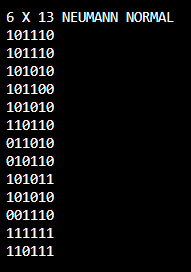
\includegraphics[width=3.5cm]{dobredane2.png}
\caption{}
\label{fig:dobredane2.png}
\end{figure}

}
\newpage
\lhead{Błędne dane}
\section{Efekt działania dla błędnych danych}
{\fontsize{14}{14}\selectfont
Program został odpowiednio zabezpieczony przed błędnymi ze strony użytkownika.

\newline

W przypadku przerwania pracy z programem spowodowanym jakimś błędem pojawi się informacja o błędzie, będzie można także, sprawdzając kod błędu (echo \$?), ustalić dokładniejszą przyczynę zakończenia działania, porównując z wartościami opisanymi w ,,helpie''.

Przykładowe błędy w programie:
\begin{itemize}
    \item Uruchomienie programu z plikiem o błędnym formacie danych (Rysunek 9).

\begin{figure}[h]
\centering
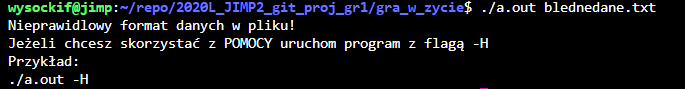
\includegraphics[width=11cm]{blednedane1.png}
\caption{}
\label{fig:blednedane1.png}
\end{figure}

\item Uruchomienie programu z błędnym argumentem po fladze \texttt{-N} (Rysunek 10).

\begin{figure}[h]
\centering
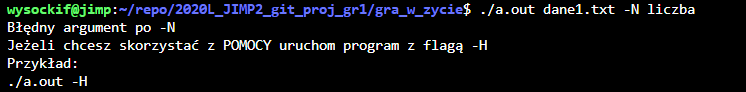
\includegraphics[width=11cm]{blednedane2.png}
\caption{}
\label{fig:blednedane2.png}
\end{figure}

\item Uruchomienie programu z nieobsługiwaną flagą (Rysunek 11).

\begin{figure}[h]
\centering
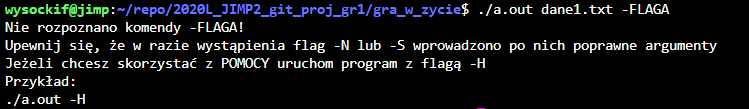
\includegraphics[width=11cm]{blednedane3.png}
\caption{}
\label{fig:blednedane3.png}
\end{figure}

\end{itemize}


}
\newpage

\lhead{Wykorzystywane narzędzia}
\section{Wykorzystywane narzędzia oraz podział prac}

{\fontsize{14}{14}\selectfont
W celu zaimplementowania programu wykorzystaliśmy poniższe narzędzia:
\begin{itemize}
\item vim
\item repozytorium git
\item debugger
\item valgrind
\item make
\end{itemize}


Praca odbywała się jednocześnie:
\begin{itemize}
\item na serwerze jimp.iem.pw.edu.pl do którego łączyliśmy się za pomocą protokółu ssh
\item na systemie Windows 10 Home z subsystemem (Windows subsystem for Linux) Ubuntu 18.04 LTS
\item na systemie Ubuntu 18.04
\end{itemize}

Wykorzystaliśmy także:
\begin{itemize}
\item bibliotekę Libpng
\item fragment kodu pngexample.c z ISODa.

\end{itemize}
Podział prac:


Bartosz odpowiadał za zapis do pliku wyjściowego, testy, helpa, Makefile'a oraz specyfikacje funkcjonalną. 

Franek z kolei za odczyt z pliku wejściowego, obsługę flag i błędów, moduł odpowiadający za zmiany generacji oraz specyfikację implementacyjną.

Wspólnie natomiast za opracowanie planu, zapis do pliku png oraz sprawozdanie końcowe.

}
\newpage
\lhead{Wycieki pamięci}
\section{Badanie wycieków pamięci}
Staraliśmy się stworzyć program wolny od wycieków pamięci tzn. każda alokowana pamięć, miała być zwalniana, gdy przestawała być w użyciu.
Do badań użyliśmy programu Valgrind.

Przykłady:
\begin{itemize}
\item Uruchomienie programu bez parametrów (Rysunek 12).

\texttt{valgrind ./a.out dane1.txt}
\begin{figure}[h]
\centering
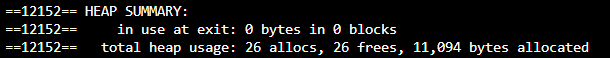
\includegraphics[width=10cm]{1.2.png}
\caption{}
\label{fig:1.2.png}
\end{figure}


\item Uruchomienie programu z parametrami (Rysunek 13).

\texttt{valgrind ./a.out dane1.txt -N 30 -S nowedane.txt}
\begin{figure}[h]
\centering
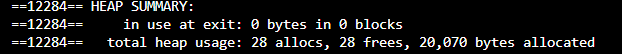
\includegraphics[width=10cm]{2.2.png}
\caption{}
\label{fig:2.2.png}
\end{figure}



Staraliśmy się także dopracować zwalnianie pamięci w przypadku błędów wynikających ze strony użytkownika.

\item Uruchomienie programu z podaniem nieistniejącego pliku (Rysunek 14).

\texttt{valgrind ./a.out nieistnieje.txt}
\begin{figure}[h]
\centering
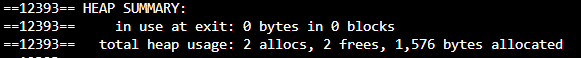
\includegraphics[width=10cm]{3.2.png}
\caption{}
\label{fig:3.2.png}
\end{figure}

\item Uruchomienie programu z plikiem, o błędnym formacie danych (Rysunek 15).

\texttt{valgrind ./a.out blednedane.txt}
\begin{figure}[h]
\centering
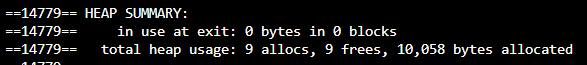
\includegraphics[width=10cm]{5.2.png}
\caption{}
\label{fig:4.2.png}
\end{figure}

\newpage
\item Uruchomienie programu z podaniem niobsługiwanej flagi (Rysunek 16).

\texttt{valgrind ./a.out dane1.txt -t}
\begin{figure}[h]
\centering
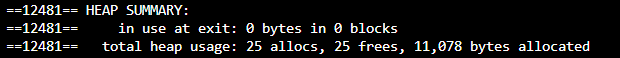
\includegraphics[width=10cm]{4.2.png}
\caption{}
\label{fig:5.2.png}
\end{figure}




\end{itemize}



\lhead{Podsumowanie i wnioski}
\section{Podsumowanie i wnioski}

{\fontsize{14}{14}\selectfont
Różnice programu końcowego, między tym co założyliśmy wynikają z nowych pomysłów i udoskonaleń. Przykładem tego może być stworzenie oddzielnej flagi wyłącznie do tworzenia obrazków z rozszerzeniem PNG, albo stworzenie funkcji ,,help''. Dzięki temu program jest łatwiejszy w obsłudze, a użytkownik ma więcej możliwości.
\newline

Wykonując ten projekt ponownie zadbalibyśmy o lepszą komunikację w zespole oraz przygotowalibyśmy precyzyjny harmonogram prac. W trakcie projektu okazało się, że oboje zajęliśmy się tą samą funkcjonalnością i musieliśmy jedną wersje odrzucić. Poza tym od razu dbalibyśmy o ,,wycieki pamięci'' i przy każdym wychodzeniu z programu sprawdzalibyśmy, czy jakaś pamięć nie została zwolniona, ponieważ sprawdzanie i poprawianie tego na końcu okazało się bardzo czasochłonne.


}
\end{document}